\documentclass[8pt]{extarticle}
\title{}
\author{Avinash Iyer}
\date{}
\usepackage[shortlabels]{enumitem}

%font setup
%
%\usepackage[math]{anttor}

%paper setup
\usepackage{geometry}
\geometry{letterpaper, portrait, margin=1in}
\usepackage{fancyhdr}

%symbols
\usepackage{amsmath}
\usepackage{amssymb}
\usepackage{hyperref}
\usepackage{gensymb}

\usepackage[T1]{fontenc}
\usepackage[utf8]{inputenc}

%chemistry stuff
\usepackage[version=4]{mhchem}
\usepackage{chemfig}

%plotting
\usepackage{pgfplots}
\usepackage{tikz}

%\usepackage{natbib}

%graphics stuff
\usepackage{graphicx}
\graphicspath{ {./images/} }

%code stuff
%when using minted, make sure to add the -shell-escape flag
%you can use lstlisting if you don't want to use minted
%\usepackage{minted}
%\usemintedstyle{pastie}
%\newminted[javacode]{java}{frame=lines,framesep=2mm,linenos=true,fontsize=\footnotesize,tabsize=3,autogobble,}
%\newminted[cppcode]{cpp}{frame=lines,framesep=2mm,linenos=true,fontsize=\footnotesize,tabsize=3,autogobble,}

\usepackage{listings}
\usepackage{color}
\definecolor{dkgreen}{rgb}{0,0.6,0}
\definecolor{gray}{rgb}{0.5,0.5,0.5}
\definecolor{mauve}{rgb}{0.58,0,0.82}

\lstset{frame=tb,
	language=Java,
	aboveskip=3mm,
	belowskip=3mm,
	showstringspaces=false,
	columns=flexible,
	basicstyle={\small\ttfamily},
	numbers=none,
	numberstyle=\tiny\color{gray},
	keywordstyle=\color{blue},
	commentstyle=\color{dkgreen},
	stringstyle=\color{mauve},
	breaklines=true,
	breakatwhitespace=true,
	tabsize=3
}
% text + color boxes
\usepackage{tcolorbox}
\tcbuselibrary{breakable}
\newtcolorbox{problem}[1]{colback = white, title = {#1}, breakable}
\newtcolorbox{solution}{colback = white, colframe = black!75!white, breakable, title = Solution}
%including PDFs
\usepackage{pdfpages}
\setlength{\parindent}{0pt}

\pagestyle{fancy}
\fancyhf{}
\rhead{Avinash Iyer}
\lhead{Problem Set 5}
\begin{document}{
  \begin{problem}{An Increase in Research Productivity}
    Suppose that the economy is on a balanced growth path in the Romer model. Then, in $2030$, research productivity $\overline{z}$ rises immediately and permanently to $\overline{z}'$.
    \begin{enumerate}[(a)]
      \item Make a graph of $y_t$ over time using a ratio scale.
      \item Why might research productivity increase in an economy?
    \end{enumerate}
  \end{problem}
  \begin{solution}
    \begin{tcolorbox}[colback = white, title = (a), breakable]
      \begin{center}
        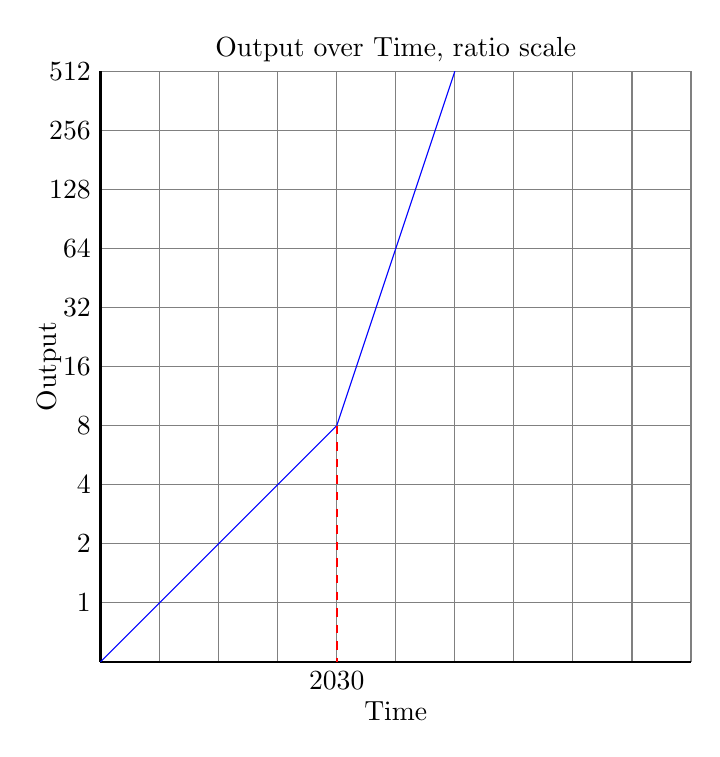
\begin{tikzpicture}[scale = 0.75]
          \draw[thin, gray] (0,0) grid (10,10);
          \draw[thick, black] (0,0) -- (0,10);
          \draw[thick, black] (0,0) -- (10,0);
          \draw[blue] (0,0) -- (4,4);
          \draw[blue] (4,4) -- (6,10);
          \draw [thick, red,dashed] (4,4) -- (4,0);
          \node [anchor = south] at (5,10) {Output over Time, ratio scale};
          \node [anchor = north] at (4,0) {$2030$};
          \node[anchor = east] at (0,1) {$1$};
          \node[anchor = east] at (0,2) {$2$};
          \node[anchor = east] at (0,3) {$4$};
          \node[anchor = east] at (0,4) {$8$};
          \node[anchor = east] at (0,5) {$16$};
          \node[anchor = east] at (0,6) {$32$};
          \node[anchor = east] at (0,7) {$64$};
          \node[anchor = east] at (0,8) {$128$};
          \node[anchor = east] at (0,9) {$256$};
          \node[anchor = east] at (0,10) {$512$};
          \node[anchor = south, rotate = 90] at (-0.5,5) {Output};
          \node[anchor = north] at (5,-0.5) {Time};
        \end{tikzpicture}
      \end{center}      
    \end{tcolorbox}
    \begin{tcolorbox}[colback = white, title = (b), breakable]
      Research productivity might increase in an economy if the government undertakes large scale investments in education or increases the prizes or patents that it provides to new research that entices different types of innovations.
    \end{tcolorbox}
  \end{solution}
  \begin{problem}{Numbers in the Romer Model}
    Suppose the parameters in the Romer model are as follows: $\overline{A}_0 = 100$, $\overline{\ell} = 0.1$, $\overline{z} = 1/500$, and $\overline{L} = 100$.
    \begin{enumerate}[(a)]
      \item What is the growth rate of output per person in this economy?
      \item What is the initial level of output per person? What is the level of output per person after 100 years?
      \item Suppose research share were to double. How would you answer parts (a) and (b)?
    \end{enumerate}
  \end{problem}
  \begin{solution}
    \begin{tcolorbox}[colback = white, title = (a), breakable]
      The growth rate of output is equal to the growth rate of $A$, which is equal to:
      \begin{align*}
        g_a &= \overline{z}\overline{\ell}\overline{L} \\
            &= \boxed{0.02}
      \end{align*}
    \end{tcolorbox}
    \begin{tcolorbox}[colback = white, title = (b), breakable]
      The initial level of output per person is equal to:
      \begin{align*}
        y_0 &= \overline{A}_0 (1-\overline{\ell})\\
            &= \boxed{90}\\ 
            \\
        y_{100} &= \overline{A}_0 (1-\overline{\ell})(1 + \overline{z}\overline{\ell}\overline{L})^{100}\\
                &= \boxed{652}
      \end{align*}
    \end{tcolorbox}
    \begin{tcolorbox}[colback = white, title = (c), breakable]
      If research share were to double, we would get the following results:
      \begin{align*}
        g_a &= \overline{z}\overline{\ell}\overline{L}\\
            &= 0.04 \\
            \\
        y_0 &= \overline{A}_0 (1-\overline{\ell}) \\
            &= 80 \\
            \\
        y_{100} &= \overline{A}_0 (1-\overline{\ell})(1 + \overline{z}\overline{\ell}{\overline{L}})^{100} \\
                &= 4041
      \end{align*}
    \end{tcolorbox}
  \end{solution}
  \begin{problem}{A Variation of the Romer Model}
    Consider the following variation:
    \begin{align*}
      Y_t = A_t^{1/2}L_{yt}\\
      \Delta A_t = \overline{z}A_tL_{at}\\
      L_{yt} + L_{at} = \overline{L}\\
      L_{at} = \overline{\ell}\overline{L}
    \end{align*}
    There is only a single difference: we have changed the exponent on $A_t$ in the production of the output good so there is now a diminishing product to new ideas in that sector.
    \begin{enumerate}[(a)]
      \item Provide an economic interpretation for each equation.
      \item What is the growth rate of knowledge in this economy?
      \item Solve for the level of output per person at each point in time.
      \item What is the growth rate of output per person in this economy?
    \end{enumerate}
  \end{problem}
}\end{document}
